%appendix blhablhaakljfdldskj
%Created MB 03-01

\section{Muon Mass Calibration}

For heavy ($\mu$ and heavier) charged particles passing through
matter, the amount of energy deposited depends on the incident
momentum of the particle. The relationship is given by the Bethe-Block
equation \cite{bichsel}:

\begin{equation}
-\frac{dE}{dx} = Kz^2\frac{Z}{A}\frac{1}{\beta^2}\left[\frac{1}{2}ln\frac{2m_ec^2\beta^2\gamma^2T_max}{I} - \beta^2 - \frac{\delta(\beta\gamma)}{2}\right]
\end{equation}

where $\beta = v/c$ and $\gamma = 1/\sqrt{1 - \frac{v_{\mu}^2}{c^2}}$
are of the incoming particle, and the other parameters are constants
or properties of the material.

The 

\begin{figure}[h]
\begin{center}
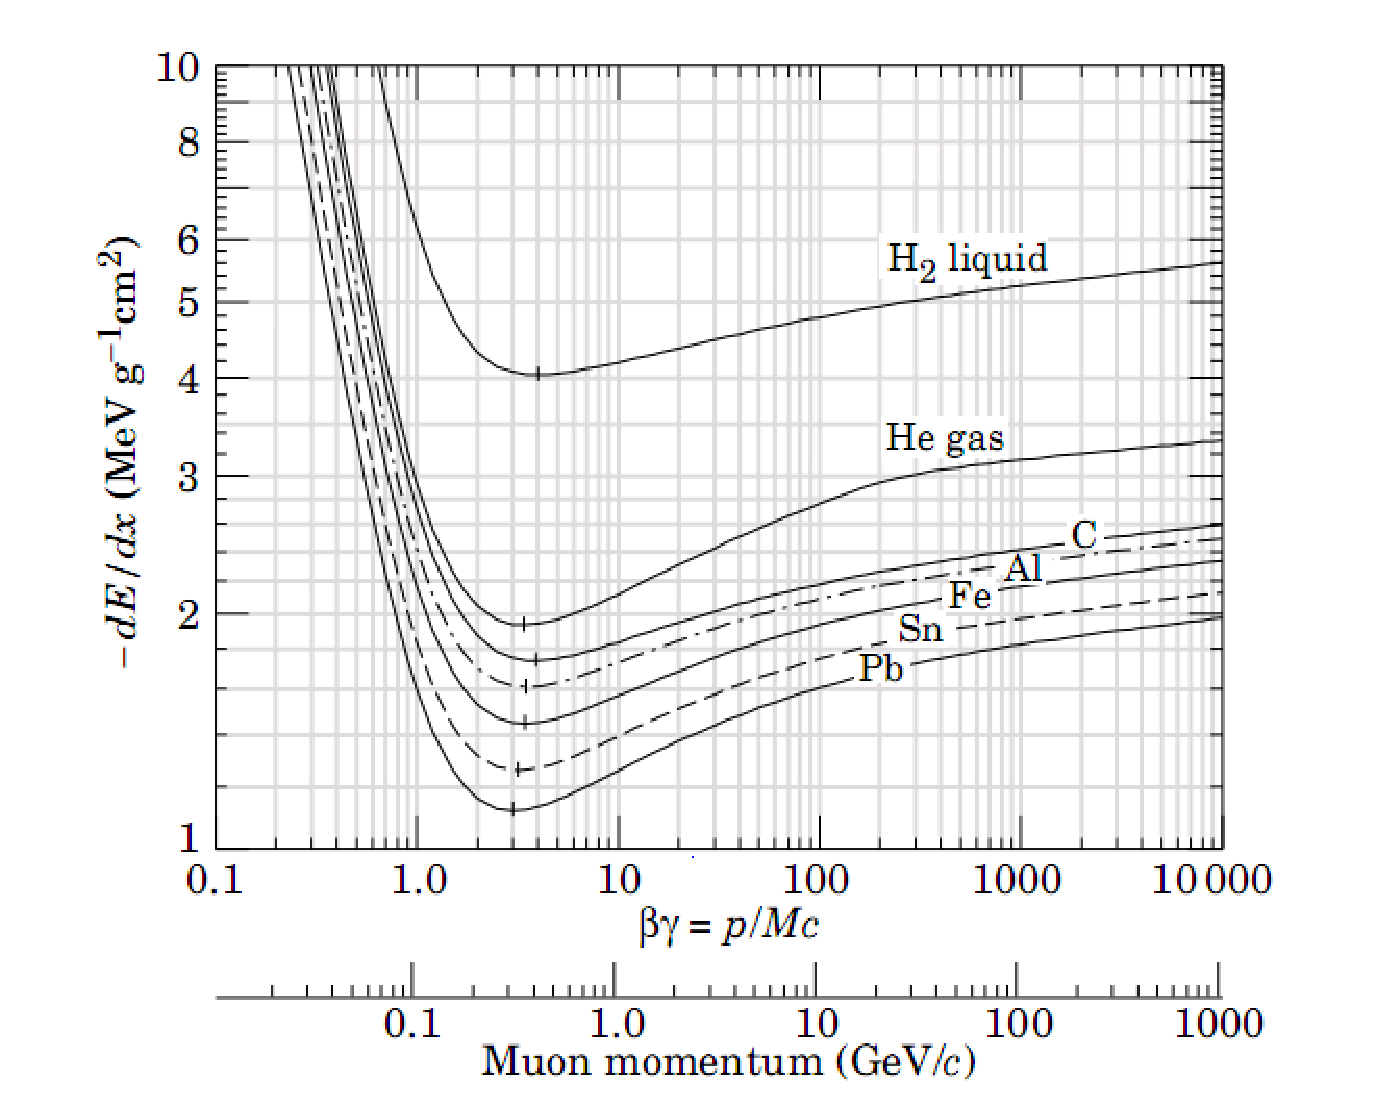
\includegraphics[width = 140mm]{figures/energy_loss.eps}
\caption{\small{Mean energy loss in various materials. In our
experiment, the scintillator consisted of carbon and hydrogen, so the
minumum ionization energy was determined by weighing the C and H
values according to mass ratio \cite{bichsel}.}}
\label{energy_loss}
\end{center}
\end{figure}
